
\documentclass[titlepage]{article}
 \usepackage[utf8]{inputenc}
\usepackage{listings}
\usepackage{hyperref}
\usepackage{float}
\usepackage{graphicx}
\usepackage{subfig}
\graphicspath{ {imagenes/} }
 \usepackage{xcolor}
 \definecolor{RoyalBlue}{cmyk}{1, 0.50, 0, 0}

\lstset{language=Java,
	keywordstyle=\color{RoyalBlue},
	basicstyle=\scriptsize\ttfamily,
	commentstyle=\ttfamily\itshape\color{gray},
	stringstyle=\ttfamily,
	showstringspaces=false,
	breaklines=true,
	frameround=ffff,
	frame=single,
	rulecolor=\color{black}}


 

% Datos de la portada
\begin{document}
	\begin{titlepage}
		\begin{center}
			\vspace*{1cm}
			\date{} % para que no aparezca la fecha la dejo en blanco
			\Huge
			\textbf{Practica 3}
			
			\vspace{0.5cm}
			\LARGE
			Aprendizaje Automático
			
			\vspace{1.5cm}
			
			\textbf{José Manuel Pérez Lendínez}
			

			
		\end{center}
	\newpage
	\tableofcontents
	\newpage
	\end{titlepage}

	\section{Digits Data Set}	
	\subsection{Comprender el problema a resolver.}
	Los datos almacenados en el dataset pertenecen a un conjunto de dígitos manuscritos. 
	Para el reconocimiento de los dígitos se utiliza una matriz de 32x32 inicialmente. Esta matriz se dividirá en matrices mas pequeñas de 4x4 sin solaparse. A cada una de estas matrices le daremos un valor numérico en el rango [0,16].
	Vamos a poner un pequeño ejemplo. La matriz inicial 32x32 seria la siguiente.
\begin{figure}[H]
	\centering
	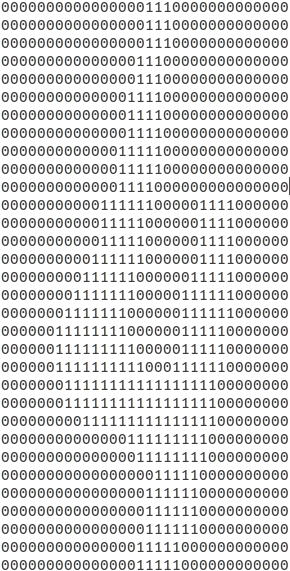
\includegraphics[width=0.7\linewidth, height=0.72\textheight]{4}

\end{figure}
	Como se ve los 0 representa la parte sin utilizar y los 1 la parte donde se escribe. 
	\newpage
	Esta matriz se divide en pequeñas matices 4x4 como en la siguiente imagen.
	\begin{figure}[H]
		\centering
			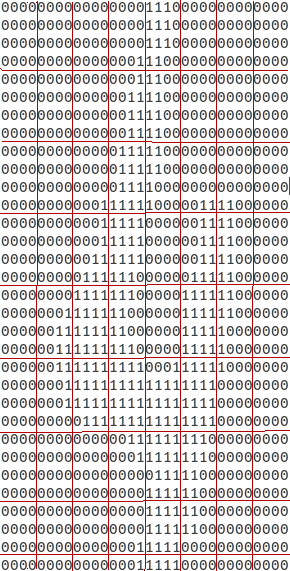
\includegraphics[width=0.7\linewidth, height=0.72\textheight]{4matriculado}

	\end{figure}
	\newpage
	En cada matriz 4x4 contaremos el numero de 1 que tenemos y le daremos ese valor. Vamos a realizar esto con la quinta fila para ver un ejemplo. 
	\begin{figure}[H]
		\centering
		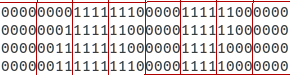
\includegraphics[width=0.7\linewidth]{columanasinmodificar}
	\end{figure}
	Esta fila de la matriz quedaría de la siguiente manera.
	\begin{figure}[H]
		\centering
		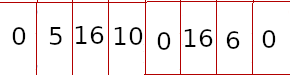
\includegraphics[width=0.7\linewidth]{columanmodificada}
		\caption{}
		\label{fig:columanmodificada}
	\end{figure}
	
	
	 Por tanto finalmente obtendremos por cada dígito manuscrito una matriz 8x8 que contendrán un valor numérico entre [0,16]. Esto es un total de 64 enteros por cada dígito analizado. La división de la matriz inicial en matrices mas pequeñas nos asegura que el tamaño del problema se mucho menor al reducir el numero de valores por cada muestra y que al tener en cuenta matrices de 4x4 para dar un valor evitamos muchas invarianzas a pequeñas distorsiones que se podrían dar si usáramos directamente la matriz de 32x32. 
	
	Las clases para los dígitos vienen dada por los números naturales de un único dígito ([0-9]), teniendo un total de 10 posibles clases.
	
	La base de datos seleccionada ya nos da la partición de train y test con el siguiente numero de instancias y participantes.
	
	\begin{table}[htbp]
		\begin{center}
			\begin{tabular}{|l|l|l|}
				\hline
				Tipo & Nº Participantes & Nº instancias \\
				\hline
				Train & 30 & 3823\\ \hline
				Text & 13 & 1797\\
				 \hline
			\end{tabular}
		\end{center}
	\end{table}

	La proporción de cada clase es muy parecida tanto en el train como en el text con una diferencia como máximo en el conjunto de entrenamiento de 13 instancias entre la clase que mas tiene y la que menos. En el caso del test la diferencia máxima es de 9 instancias. 
	
		\begin{table}[htbp]
		\begin{center}
			\begin{tabular}{|l|l|l|}
				\hline
				Clase & Nº instancias train & Nº instancias test\\
				\hline
				0 & 376 & 178\\ 
				\hline
				1 & 389 & 182\\ 
				\hline
				2 & 380 & 177\\ 
				\hline
				3 & 389 & 183\\ 
				\hline
				4 & 387 & 181\\ 
				\hline
				5 & 376 & 182\\ 
				\hline
				6 & 377 & 181\\ 
				\hline
				7 & 387 & 179\\ 
				\hline
				8 & 380 & 174\\ 
				\hline
				9 & 382 & 180\\ 
				\hline
			\end{tabular}
		\end{center}
	\end{table}
	\newpage
	
	\subsection{Preprocesado de datos}
	En este caso el he realizado una normalización muy sencilla, al saber que los datos están en el rango [0sklearn.preprocessing.PolynomialFeatures
	
	-16], solo tenemos que dividir los datos entre 16.
	
	También se ha realizado una eliminación de variables que no aportan al problema. Estas variables son aquellas en cuya columna los datos tengan una varianza menor a 0 en este caso(todas las variables que solo tienen un único valor en todas las muestras.). Para esto he utilizado la función de VarianceThreshold de sklearn.feature\_selection.
	Esto nos ahorra 2 variables que tienen una varianza de 0. Estas partes de la matriz nunca han sido utilizadas para ningún numero.
	
	Para esto utilizo la siguiente función:
	\begin{lstlisting}
def eliminarDatosVarianza(train_x,train_y,limite):
	row_train = np.size(train_X,0)
	
	datos = np.concatenate((train_X, test_X), axis=0)
	
	selector = VarianceThreshold(limite)
	datos_procesados = selector.fit_transform(datos)
	
	train = datos_procesados[:row_train, :]
	test = datos_procesados[row_train:, :]
	return train,test
	\end{lstlisting}
	
A continuación vamos a añadir nueva información que nos ayude a clasificar, para esto uso la librería sklearn.preprocessing.PolynomialFeatures con el parámetro de grado 2. El código de la función seria el siguiente.
\begin{lstlisting}
def anadirInformacionPolinomial(train_X, test_X, grado = 2):
	poly = PolynomialFeatures(grado)
	train_X = poly.fit_transform(train_X)
	test_X = poly.fit_transform(test_X)
	
	return train_X, test_X
\end{lstlisting}

Esto nos añadirá nueva información de la siguiente manera. Si partimos de una muestra con [a,b] nos daría $[1,a,b,a^2,ab,b^2]$. En este caso he optado por elegir 2 porque con 4 la memoria se desborda al añadir demasiada información y con 3 no me mejoro el problema.

\subsection{Selección de clase de funciones a usar.}

El problema al que nos enfrentamos es un problema de clasificación. Vamos a usar una función lineal para solucionar este problema. Al ser clasificación y tener mas de dos etiquetas este problema no puede ser solucionado con una función lineal unicamente. Para esto utilizaremos la función lineal enfrentando una clase a todas las demás(one vs rest). 

Vamos a poner un pequeño ejemplo con tres clases para ver como funcionaria. Como se ve en la siguiente imagen es imposible dividir las clases con una única linea. 
\begin{figure}[H]
	\centering
	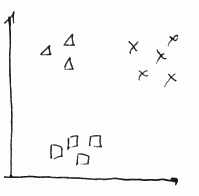
\includegraphics[width=0.7\linewidth]{screenshot002}
	\caption{Conjunto de clases}
	\label{fig:screenshot002}
\end{figure}

En las siguientes imágenes se ve como enfrentamos una clase a las otras dos de forma que si se puede conseguir una separación mediante una función lineal.



\begin{figure}[H]
	\centering
	\subfloat[Triangulos]{
		\label{f:gato}
		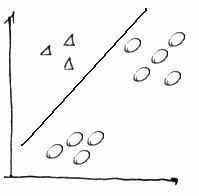
\includegraphics[width=0.3\textwidth]{screenshot001}}
	\subfloat[Cuadrados]{
		\label{f:tigre}
		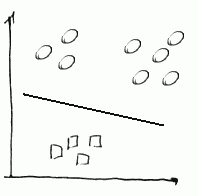
\includegraphics[width=0.3\textwidth]{screenshot004}}
	\subfloat[Cruces]{
		\label{f:conejo}
		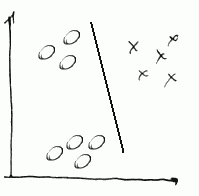
\includegraphics[width=0.3\textwidth]{screenshot005}}
	\caption{División mediante one vs rest}
\end{figure}

Por tanto nos quedaremos con las funciones lineales para este problema.
 
\subsection{Definición de training, validación y test.}
En este caso los datos vienen divididos ya en train y test. En el train se tienen 40 personas y el test 13. Si somos capaces de conseguir un buen $E_{out}$, estaremos consiguiendo que sea capaz de reconocer los números sin tener en cuenta la forma de escribir de cada participante. Esto me parece la mejor opción y no he realizado ninguna modificación en este apartado.

\subsection{Necesidad de regularización}
Como se explico en teoría la regularización nunca viene mal para eliminar un poco de sobreajuste de nuestro modelo. En este caso he utilizado la regularización l1 (usa el valor absoluto) puesto después de varias pruebas me ha dado mejores resultados que l2(usa pesos al cuadrado). En este caso la diferencia es muy pequeña llegando a alrededor de un 1\%. Pero al ser también mas eficiente y rápida la regularización l1 he terminado optando por esta.

\subsection{Definición del modelos a usar y sus parámetros}
Vamos a utilizar dos algoritmos que utilizan funciones lineales. Uno sera regresión logistica y el otro perceptron. Los dos se basan en one vs rest(ovr) para resolver problemas multiclase.
\begin{enumerate}
	\item{Perceptron}: En este caso es el mas sencillo de los dos puesto que solo tenemos que ajustar tres parametros sencillos de entender. Usaremos la implementación de la librería sklearn.linear\_model.Perceptron
	\begin{enumerate}		
		\item{Umbral de parada:} Indicara cuando tengamos un error menor al indicado pararemos el perceptron.
		\item{Numero de iteraciones sin cambio:} Como el propio nombre indica cuando se realizen un numero de iteraciones en las que no conseguimos mejorar, el perceptron parara la ejecución.
		\item{Numero de iteraciones máxima:} En este caso sera en numero máximo de iteraciones que el perceptron  podrá realizar si no decide parar antes por alguna de las dos variables explicadas anteriormente.
	\end{enumerate}
	El perceptron intentara separar una clase del resto mediante un hyperplano. 
	
	\item{Regresión logística:} En este caso es tenemos los mismos parámetros que el perceptron solo tenemos dos parámetros que coinciden con los dados para el perceptron.
	\begin{enumerate}		
		\item{Umbral de parada:} Indicara cuando tengamos un error menor al indicado pararemos el perceptron.
		\item{Numero de iteraciones máxima:} En este caso sera en numero máximo de iteraciones podrá realizar si no decide parar antes por el umbral de parada.
	\end{enumerate}
	Regresión lineal intenta estimar la probabilidad de que pertenezca a una de las clases o al resto. Requiere grandes tamaños de datos y es muy eficiente y no requiere grandes recursos computacionales.
\end{enumerate}

\subsection{Selección y ajuste del modelo final}
Los datos medidos para los dos algoritmos con los parametros por defecto dados por la librería sklearn son los siguientes.
	\begin{table}[H]
		\begin{center}
			\begin{tabular}{|l|l|l|}
				\hline
				Algoritmo & Tiempo & Eout\\
				\hline
				Perceptron & 0.6093 & 4.0066\%\\ 
				\hline
				Regresión logística & 4.9787 & 2.5041\%\\  
				\hline
			\end{tabular}
		\end{center}
	\end{table}
El ajuste con regresión logística es un 1.5\% mejor aunque el perceptron es mas rápido que regresión logística. En este caso voy a optar por elegir el modelo de regresión logística para tratar de bajar el Eout por debajo del 2\%. Realizo esta selección para intentar mejorar el 98.00\% tasa de acierto que consigue k-nn con k=1 en estos datos. La tasa de acierto de k-nn viene especificada en el fichero optdigits.name del dataset. Los resultados que muestra son los siguientes.
\begin{figure}[H]
	\centering
	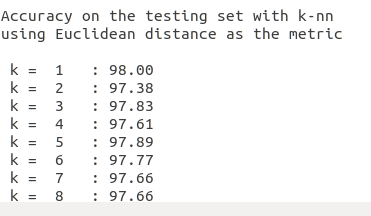
\includegraphics[width=0.7\linewidth]{screenshot006}
\end{figure}
 
\subsection{Métrica usada}
La métrica usada en este caso es la tasa de acierto(Accuracy) que se basa en calcular el numero de aciertos totales tenidos entre el total de muestras. 


$$
Accuracy=\frac{Numero\ correcto\ de\ prediciones}{Numero\ total\ de\ predicciones}
$$
Me he decidido por esta métrica porque lo importante en este problema es ser capaces de acertar el numero. Para esto lo mejor es ver si la predicción realizada por regresión logística acertó con la etiqueta dada para esa entrada.

\subsection{Estimación del error Eout}
En este apartado vamos a ver cuanto he conseguido mejorar los datos dados por la regresión logística con los parámetros por defecto del algoritmo dado por sklearn.
En este caso me centre en mejorar mediante la regularización. Comparando si para nuestro problema cual es el parámetro C mejor. Este parámetro nos fuerza a regularizar de forma mas fuerte conforme mas bajo sea. 
\begin{figure}[H]
	\centering
	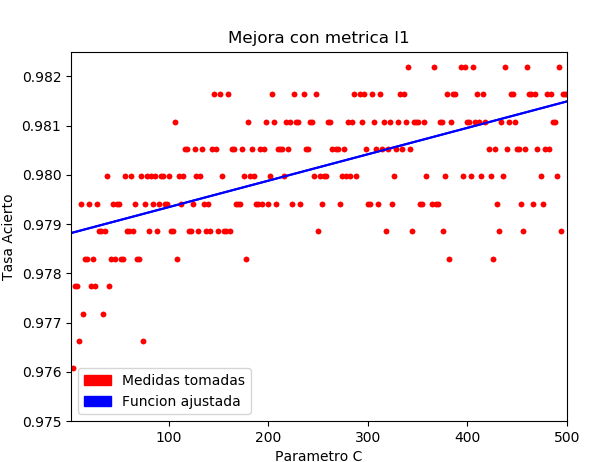
\includegraphics[width=0.7\linewidth]{screenshot007}
\end{figure}
Como se ve en la grafica a partir  de 300 en c empezamos a sobrepasar el 98\% de tasa de acierto que conseguía el k-nn con k = 1.

Con el parámetro 500 obtengo un Eout 1.8363939899833093\%.
Para esto el parámetro umbral de parada lo asigno a $1e-3$ y las iteraciones máximas a 100.

\subsection{Discutir y justificar la calidad del modelo obtenido.}
El modelo encontrado me parece muy bueno siendo capaz de superar el 98\% de acierto y con un tiempo de poco mas de 2.7 segundos mejorando también el tiempo que nos dio por defecto en las pruebas anteriores que fue de 5 segundos.
Vamos a mostrar una matriz de confusión para ver los resultados.
\begin{figure}[H]
	\centering
	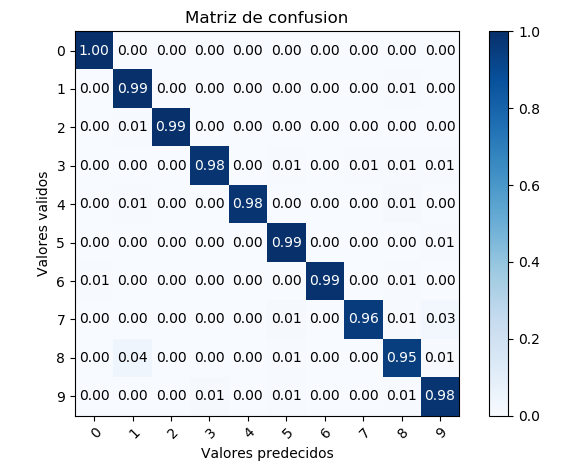
\includegraphics[width=0.7\linewidth]{screenshot009}

\end{figure}

Como se ve la diagonal es la que tiene el peso de los aciertos y fuera de esta apenas hay un par de valores en los que nuestro algoritmo falla. Estos valores donde falla nos están diciendo que confundimos en algunos casos los 8 con 1 y los 7 con 9. 



\section{Airfoil self noise}
\subsection{Comprender el problema a resolver}
Este conjunto de datos contiene los resultados de las pruebas aerodinámicas de la NASA en 1989. El dataset mide el ruido causado por el flujo de aire sobre una superficie aerodinámica. Este campo de investigación es conocido como aeroacústica. Estos resultados están medidos en un túnel de viento. Se prueban los perfiles aerodinámicos de diferentes tamaños con varias velocidades de viento y distintos ángulos. La duración del perfil aerodinámico y la posición del observador fueron las mismas en todos los experimentos.

El dataset contiene las siguientes variables:
\begin{enumerate}
	\item Frecuencia en hercios.
	\item Ángulo de ataque en grados.
	\item Longitud de la cuerda en metros
	\item Velocidad de flujo libre en metros por segundo
	\item Espesor de desplazamiento lateral de aspiración en metros
\end{enumerate}

La etiqueta a adivinar en este caso es un numero real que representara el nivel de presión sonora escalonado. Por tanto no se trata de un conjunto de etiquetas finito, sino que es un numero real. Esto complicara el problema. 
El datase se compone de 1503 muestras

Como en este caso tenemos pocas variables en el dataset, podremos buscar una correlación entre la variable a predecir y las demás variables. Esto nos podría ayudar a la hora de mejorar la predicción. Para esto vamos a mostrar una matriz de correlación donde tendremos las variables del problema y la clase. La clase sera la ultima columna y las variables estarán ordenadas como se explicaron anteriormente.
\begin{figure}[H]
	\centering
	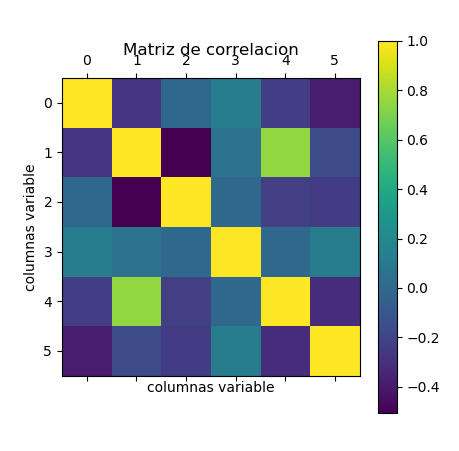
\includegraphics[width=0.7\linewidth]{screenshot010}

\end{figure}

En este caso como se ve en el gráfico no hay ninguna variable que nos ayude. Por tanto no podemos ver ninguna variable que tenga una relación con la clase. 

\subsection{Preprocesado de datos}
En este ejemplo realizaremos dos procesamientos con los datos. 
El primero sera la normalización de los datos. Para esto como no se tienen números negativos en la muestra podremos buscar el máximo de cada columna y utilizar este unicamente para la normalización.

\begin{lstlisting}
def normalizacionMax(datos):
	datos = datos/datos.max(axis=0)   
	return datos
\end{lstlisting}

El segundo paso que realizaremos con los datos sera añadir nueva información que nos ayude a clasificar, para esto realizare lo mismo que en el caso problema anterior añadiendo nueva información. En este caso al tener un numero de variables mas pequeño podemos meter mas información sin tener problemas de memoria. En este caso y tras algunas pruebas me he decidido por meter información de grado 4. Con esto he conseguido disminuir mejor hasta un 30\% que en el caso de no meter información.

\begin{lstlisting}
def anadirInformacionPolinomial(train_X, test_X, grado = 2):
	poly = PolynomialFeatures(grado)
	train_X = poly.fit_transform(train_X)
	test_X = poly.fit_transform(test_X)
	
	return train_X, test_X
\end{lstlisting}

En este caso no vamos a eliminar datos por varianza como en el apartado anterior puesto que no tenemos una gran cantidad de variables como en el ejercicio anterior y ninguna repite todos sus valores.

\subsection{Seleccion de la clase de funciones a usar}
En este caso nos enfrentamos a un problema de predicción en el que tendremos que predecir el valor de la etiqueta y de nuestra muestra. Se utilizara la familia de funciones lineales intentando ajustar la función lo mejor posible a los puntos para tener el menor error a la hora de predecir la etiqueta.

\subsection{Definición de training, validación y test}
En este caso voy a dividir los datos en un 80\% para el trainig y un 20\% para el test. La división lo realizaremos de forma aleatoria para no estar condicionados por el orden en el que nos dieron los datos. Para estoy utilizare la librería sklearn.model\_selection.train\_test\_split.

\begin{lstlisting}
def dividirTrainTest(X,y, tam_test = 0.2):
	X_train, X_test, y_train, y_test = train_test_split(X, y, test_size=tam_test, random_state=42)
	return X_train, X_test, y_train, y_test
\end{lstlisting}

\subsection{Necesidad de regularización}
Puesto que al añadir información de grado 4 he metido muchas mas variables al problema, podremos utilizar la regularización L2, que produce en general valores de peso más pequeños, lo que estabiliza las ponderaciones. Aunque en este caso nuestro modelo no se ajusta muy bien a a los datos y no obtendremos mejoras considerables.

\subsection{Definición de los modelos a usar y sus parámetros}
En este caso el modelo a usar sera regresión lineal. De los dados en practicas es es el único que puede afrontar este problema de predicción. He utilizado la implementación de la librería sklearn.linear\_model.LinearRegression. En este caso no tenemos ningún parámetro que ajustar.

\subsection{Selección y ajuste del modelo final}
En este apartado no podemos añadir nada mas puesto que regresión linear no tiene parámetros que tengamos que ajustar y es el único que podemos utilizar de los dados en practicas.

\subsection{Metrica usada}
En este caso usamos la métrica de coeficiente de determinación ($R^2$). Se calcula como $1-\frac{u}{v}$, donde u es la suma residual de cuadrados ((y\_true - y\_pred) ** 2) .sum () y v es la suma total de cuadrados ((y\_true - y\_true.mean ()) ** 2) .sum (). 

Tambien utlizaremos una segunda metrica que es una mejora de $R^2$, Estama metrica es conocida como coeficiente de determinación ajustado. Y su formala es la siguiente:
$$
	1-(1-R 2) *(n-1) /(n-p-1)
$$
En este caso n representa el numero de muestras de la partición que estemos clasificando y p el numero de características de cada muestra.

R2 tiende a estimar de forma optimista el ajuste de la regresión lineal. Siempre aumenta como el número de características que se incluyen en el modelo. R2 ajustado intenta corregir esta estimación excesiva. R2 ajustado podría disminuir si un efecto específico no mejora el modelo. 

R2 ajustado siempre es menor o igual que R2. Un valor de 1 indica un modelo que predice perfectamente valores del campo objetivo. Un valor que es menor o igual que 0 indica un modelo que no tiene ningún valor predictivo. En el mundo real, R2 ajustado se encuentra entre estos valores. 

\subsection{Estimación del error Eout}
En este caso lo que mas me a afectado a la métrica ha sido incluir mayor información al problema con el grado. Voy a mostrar en una tabla la mejora:
\begin{table}[H]
	\begin{center}
		\begin{tabular}{|l|l|l|l|}
			\hline
			Grado & Tiempo & R2& R2 ajustado\\
			\hline
			0 &  0.0082 & 55.82979\% &55.0811\\ 
			\hline
			2 &0.0098 & 68.4058\% & 66.0278\\  
			\hline
			3  & 0.0019 &  75.9331\% & 70.4096\\  
			\hline
			4  & 0.0137 & 84.0892\% & 72.5676\\  
			\hline
			5  & 0.0238 & 80.0246\% & -24.8458\\  
			\hline
		\end{tabular}
	\end{center}
Como se ve en la tabla anterior el mejor resultado se da con el grado 4 mientras que el tiempo no tiene un aumento muy considerable siendo muy rápido de ejecuta.
\subsection{Discutir y justificar el la calidad del modelo obtenido.}
Al tener un dataset en el que no tenemos clases, sino que la etiqueta y es un valor real que tendremos que acertar es mas complicado mediante regresión lineal conseguir un buen modelo para ajustar a este problema. 

En este caso se tendrá mas en cuenta la métrica R2 mejorada puesto que al añadir información al problema estamos metiendo una gran cantidad de nuevas características que en R2 nos aumentara el valor de predicción sin tener en cuenta que la cantidad de características.
Lo máximo conseguido a sido un 70\% y esto aun así se quedaran corto para asegurar que nuestros resultados serán cercanos a la etiqueta y puesto que nos podriamos estar equivocando un 30\%. Es un problema demasiado complejo para ser aproximardo con regresión lineal. Quizás tendríamos que elegir otros modelos mas avanzados como podrían ser random forest regression o XGBoost regression que podrían ajustarse mejor a este dataset.
\end{table}

\section{Bibliografía}
\subsection{Digits Data Set}


\url{https://chrisalbon.com/machine_learning/feature_selection/variance_thresholding_for_feature_selection/}
\\
\url{https://stackoverflow.com/questions/2148543/how-to-write-a-confusion-matrix-in-python}
\\

\subsection{Airfoil self noise}
\url{https://www.simonwenkel.com/2018/11/06/revisiting-ml-NASA-airfoil-noise.html}
\\
\url{https://www.ibm.com/support/knowledgecenter/es/SS4QC9/com.ibm.solutions.wa_an_overview.2.0.0.doc/rsquared_adjusted.html}
\\
\url{https://stackoverflow.com/questions/51038820/how-to-calculated-the-adjusted-r2-value-using-scikit}




\end{document}

